\section{RC Week 6}
\subsection{Mechanism behind function calling}
\begin{frame}{Memory Layout}
Before function calling we would like to first give a brief introduction to the memory organization of the system
\begin{columns}
	\column{.5\textwidth}
	\vspace{0.05in}
	
	\begin{bytefield}[leftcurly=., leftcurlyspace=0pt]{16}
		\begin{leftwordgroup}{Low}
			\bitbox{16}{Text}
		\end{leftwordgroup}\\
		\begin{leftwordgroup}{}
			\bitbox{16}{Consts}
		\end{leftwordgroup}\\
		\begin{leftwordgroup}{}
		\bitbox{16}{Statics}
		\end{leftwordgroup}\\
		\begin{leftwordgroup}{High}
			\wordbox[lrt]{1}{Heap $\downarrow$} \\
			\skippedwords \\ 
			\bitbox[lrb]{16}{Stack $\uparrow$}
		\end{leftwordgroup}\\
	\end{bytefield}
	
	* This graph is up-side-down. 
	
	\column{.5\textwidth}
	\vspace{0.05in}
	\structure{Explanation}
	\begin{itemize}
	\item ``Text", just ``code"
	\item ``consts", not like \texttt{const int const}, but string literals, \texttt{"Hello world"}.
	\item ``Statics", global variables, static variables in functions. ``static" refers to lifetime.
	\item ``Heap", where you \texttt{new}.
	\item ``Stack", everything local. Arugments, return values, return addresses ...
	\end{itemize}
\end{columns}
\end{frame}

\begin{frame}[fragile]{Element in a stack}
\begin{columns}
	
	\column{.5\textwidth}
	\vspace{-0.15in}
	
	\begin{bytefield}[leftcurly=., leftcurlyspace=0pt]{16}
		\begin{leftwordgroup}{}
			\bitbox{16}{z = 4 @ foo(3)}
		\end{leftwordgroup}\\
		\begin{leftwordgroup}{}
			\bitbox{16}{x = 3 @ foo(3)}
		\end{leftwordgroup}\\
		\begin{leftwordgroup}{}
			\bitbox{16}{Ret = ?}
		\end{leftwordgroup}\\
		\begin{leftwordgroup}{\texttt{foo}}
		\bitbox{16}{RA = \&CALLS + 1}
		\end{leftwordgroup}\\
		\begin{leftwordgroup}{}
			\bitbox{16}{q = ? @ main()}
		\end{leftwordgroup}\\
		\begin{leftwordgroup}{}
			\bitbox{16}{p = 3 @ main()}
		\end{leftwordgroup}\\
		\begin{leftwordgroup}{\texttt{main}}
			\bitbox{16}{...}
		\end{leftwordgroup}
	\end{bytefield}
	\column{.5\textwidth}
	\vspace{-0.2in}
\begin{minted}{c++}
int foo(int x) {
    int z = x + 1;
    /* Here */ 
    return z + x;  
}
int main() {
    int p = 3;
    p = foo(p); // <- CALLS
    int q = 10;
}
\end{minted}
\end{columns}
\vspace{0.1in}
The stack maintains the following information
\begin{itemize}
	\item Function arguments. They are evaluated and on to the stack.
	\item Local variables (arrays). They are reserved before initialized.
	\item Return value and return address. Return address tells which instruction to pick up when the call returned.
\end{itemize}
\end{frame}

\begin{frame}{Remarks}
\begin{block}{Calling mechanism is about \textit{Abstraction}}
	Calling mechanism is designed in such way to support procedural abstraction. In order for the abstraction to work, we require
	\begin{center}
		\structure{Each function call is independent}
	\end{center}
	This is especially important if you have recursion calls.
\end{block}

\begin{block}{Calling mechanism is platform dependent}
	\begin{itemize}
		\item Calling mechanism is neither specified by standard, nor unique!
		\item Whose responsibility to manage arguments? Caller / callee?
		\item Compiler might optimize unused variables out.
		\item Compiler might use register to store information.
		\item Compiler is allowed optimize the entire stack frame out.
	\end{itemize}
\end{block}
\end{frame}

\begin{frame}{Puzzles for \alert{FFFUUUNNNNN}!}
Understanding calling stack is most useful in finding out what has gone wrong when you observe strange behavior of your program. This is very much like solving puzzles.

We now give you a few such puzzles to entertain you. Note all the code we gave you below contains \alert{undefined behaviors} so don't be surprised if you cannot reproduce this problem.

This is actually worth noting. Many undefined behaviors would cause different behavior since given different situation on the stack. 

\begin{itemize}
	\item This code works on my computer but crashed on OJ.
	\item This code crashes / malfunctions if I change unrelated things.
	\item Student: ``TA, my code can't work!". \\
	      TA\qquad: ``Can you demo? I can't reproduce your problem"\\
	      Student: ``Suddenly I can't Either! But it crashes on OJ!"
	\item This code randomly crashes.
\end{itemize} 
\end{frame}

\begin{frame}[fragile]{Puzzle 0: Why not VLA?}
\textit{Variable Length Arrays} (VLA) are arrays whose size are determined at compile time. For example in the following code \texttt{arrX} is a VLA, and \texttt{arrY} is a usual array.
\begin{minted}{c}
void foo() {int t = 20; int arrX[t * t]; int arrY[400];}
\end{minted}
But both C++ and C choose \textbf{not} to support this language feature (above code won't compile). Explain what's the underlying reason.

\pause
\begin{block}{Explanation}
What would be the impact of this feature? Variable length array will consume variable amount of memory.

If the array is a local variable. The stack frame size of the function cannot be determined in compile time. 

The need to know the size of a function's compile time stack frame size is centric in language design. 
\end{block}      `
\end{frame}

\begin{frame}[fragile]{Puzzle 1: Orders matter}
\texttt{$-->$ code/rc5pz1/a.cpp}
\inputminted{c++}{code/rc5pz1/a.cpp}
User inputed \texttt{Hello}, symptoms are:
\begin{itemize}
	\item Program crashes after printing 3 times of \texttt{Hello} strangely.
	\item Program runs fines if change input to \texttt{Bad}.
	\item Program doesn't crash if switch \texttt{char a[4]} and \texttt{int x = 4}. But the program keeps printing \texttt{Hellx} (x decreasing char in ascii).
\end{itemize}
\end{frame}

\begin{frame}{Solution 1}
\begin{columns}
	\column{.5\textwidth}
	
	\begin{bytefield}[leftcurly=., leftcurlyspace=0pt]{16}
		\begin{leftwordgroup}{4B}
			\bitbox{16}{s.x = 4 @ foo()}
		\end{leftwordgroup}\\
		\begin{leftwordgroup}{1B}
			\bitbox{16}{s.a[0]  @ foo()}
		\end{leftwordgroup}\\
		\begin{leftwordgroup}{1B}
			\bitbox{16}{s.a[1]  @ foo()}
		\end{leftwordgroup}\\
		\begin{leftwordgroup}{1B}
			\bitbox{16}{s.a[2]  @ foo()}
		\end{leftwordgroup}\\
		\begin{leftwordgroup}{1B}
			\bitbox{16}{s.a[3]  @ foo()}
		\end{leftwordgroup}\\
		\begin{leftwordgroup}{\texttt{foo}}
			\bitbox{16}{RA = !!}
		\end{leftwordgroup}\\
		\begin{leftwordgroup}{\texttt{main}}
			\bitbox{16}{...}
		\end{leftwordgroup}
	\end{bytefield}
	
	Return address is corrupted.
	
	\column{.5\textwidth}
	
	\begin{bytefield}[leftcurly=., leftcurlyspace=0pt]{16}
		\begin{leftwordgroup}{1B}
			\bitbox{16}{s.a[0]  @ foo()}
		\end{leftwordgroup}\\
		\begin{leftwordgroup}{1B}
			\bitbox{16}{s.a[1]  @ foo()}
		\end{leftwordgroup}\\
		\begin{leftwordgroup}{1B}
			\bitbox{16}{s.a[2]  @ foo()}
		\end{leftwordgroup}\\
		\begin{leftwordgroup}{1B}
			\bitbox{16}{s.a[3]  @ foo()}
		\end{leftwordgroup}\\
		\begin{leftwordgroup}{4B}
			\bitbox{16}{s.x = !! @ foo()}
		\end{leftwordgroup}\\
		\begin{leftwordgroup}{\texttt{foo}}
			\bitbox{16}{RA = \&main + 1}
		\end{leftwordgroup}\\
		\begin{leftwordgroup}{\texttt{main}}
			\bitbox{16}{...}
		\end{leftwordgroup}
	\end{bytefield}

	Variable \texttt{s.x} is corrupted.
\end{columns}

\vspace{1ex}

C99 §6.7.2.1 clause 13 states: Within a structure object, the non-bit-field members and the units in which bit-fields reside have addresses that increase in the order in which they are declared.

\end{frame}

\begin{frame}[fragile]{Puzzle 2: Missing return value?}
\texttt{$-->$ code/rc5pz2/a.cpp}
\inputminted{c++}{code/rc5pz2/a.cpp}
This code is supposed to keeping squaring a number until it's greater than 100, but the real symptoms are
\begin{itemize}
	\item Program output random number if c/with \texttt{g++ a.cpp}
	\item Program always return 225 if c/with \texttt{g++ -O1 a.cpp}
	\item Program spits random number if c/with \texttt{g++ -O1 a.cpp}, if we change ``\texttt{foo(x);}" to ``\texttt{y = foo(x);}".
\end{itemize}
\end{frame}

\begin{frame}{Solution 2}
\begin{columns}
	\column{.5\textwidth}
	
	\begin{bytefield}[leftcurly=., leftcurlyspace=0pt]{16}
		\begin{leftwordgroup}{}
			\bitbox{16}{x = 225  @ foo(225)}
		\end{leftwordgroup}\\
		\begin{leftwordgroup}{}
			\bitbox{16}{Ret = 225}
		\end{leftwordgroup}\\
		\begin{leftwordgroup}{\texttt{foo}}
			\bitbox{16}{RA = \&foo(15)}
		\end{leftwordgroup}\\
		\begin{leftwordgroup}{}
			\bitbox{16}{x = 225  @ foo(15)}
		\end{leftwordgroup}\\
		\begin{leftwordgroup}{}
			\bitbox{16}{Ret = ?}
		\end{leftwordgroup}\\
		\begin{leftwordgroup}{\texttt{foo}}
			\bitbox{16}{RA = \&main}
		\end{leftwordgroup}\\
		\begin{leftwordgroup}{\texttt{main}}
			\bitbox{16}{...}
		\end{leftwordgroup}
	\end{bytefield}
	
	Without optimization
	\column{.5\textwidth}
	
	\begin{bytefield}[leftcurly=., leftcurlyspace=0pt]{16}
		\begin{leftwordgroup}{}
			\bitbox{16}{x = 225  @ foo(225)}
		\end{leftwordgroup}\\
		\begin{leftwordgroup}{}
			\bitbox{16}{Ret = 225}
		\end{leftwordgroup}\\
		\begin{leftwordgroup}{\texttt{foo}}
			\bitbox{16}{RA = \&main}
		\end{leftwordgroup}\\
		\begin{leftwordgroup}{\texttt{main}}
			\bitbox{16}{...}
		\end{leftwordgroup}
	\end{bytefield}
	
	After optimization
\end{columns}
\end{frame}

\begin{frame}[fragile]{Puzzle 2.5: Who moved my cheese?}
\texttt{$-->$ code/rc5pz25/a.cpp}
\inputminted{c++}{code/rc5pz25/a.cpp}

We observe the output to be \texttt{-1}. However we haven't changed the variable \texttt{cheese}. Who \texttt{mov}-ed my \texttt{cheese}.
\end{frame}

\begin{frame}{Solution 2.5}
\begin{columns}
	
	\column{.5\textwidth}
	\vspace{-0.2in}
	\begin{bytefield}[leftcurly=., leftcurlyspace=0pt]{16}
		\begin{leftwordgroup}{}
			\bitbox{16}{cheese = !! @ setFirst()}
		\end{leftwordgroup}\\
		\begin{leftwordgroup}{}
			\bitbox{16}{...}
		\end{leftwordgroup}\\
		\begin{leftwordgroup}{\texttt{setFirst}}
			\bitbox{16}{RA = \&main}
		\end{leftwordgroup}\\
		\begin{leftwordgroup}{}
			\bitbox{16}{arr[0][0]  @ main()}
		\end{leftwordgroup}\\
		\begin{leftwordgroup}{}
			\bitbox{16}{arr[0][1] @ main()}
		\end{leftwordgroup}\\
		\begin{leftwordgroup}{}
			\bitbox{16}{...  @ main()}
		\end{leftwordgroup}\\
		\begin{leftwordgroup}{}
			\bitbox{16}{arr[1][0]  @ main()}
		\end{leftwordgroup}\\
		\begin{leftwordgroup}{}
			\bitbox{16}{...  @ main()}
		\end{leftwordgroup}\\
		\begin{leftwordgroup}{}
			\bitbox{16}{Ret = ?}
		\end{leftwordgroup}\\
		\begin{leftwordgroup}{}
			\bitbox{16}{RA = ...}
		\end{leftwordgroup}\\
		\begin{leftwordgroup}{\texttt{main}}
			\bitbox{16}{...}
		\end{leftwordgroup}
	\end{bytefield}
	\column{.5\textwidth}
	
	\begin{itemize}
		\item The loop out-of-bound.
		\item How 2D arrays are stored.
		\item Understand how indexing works.
		\item We omit the arguments and return values of \texttt{foo} on the graph
	\end{itemize}
\end{columns}
\end{frame}

\begin{frame}[fragile]{Puzzle 3: A hijack}
For this puzzle to work you might need to turn off \textit{Address Space Layout Randomization} and set \texttt{-fno-stack-protector} in g++.

\texttt{$-->$ code/rc5pz3/a.cpp}
\inputminted{c++}{code/rc5pz3/a.cpp}

The trick is a carefully constructed input:
\begin{center}
 \texttt{voidsecretFunction2e34!2\&\&Q.\%x;"]}
\end{center}
We observe the output is \texttt{You shouldn't be here...}

The question is how does this happen, since \texttt{secretFunction} is not called at all?
\end{frame}

\begin{frame}[fragile]{Stack unwinding / unrolling}
Hope you still remember \textit{constructors} and \textit{destructors}!

When the function returns, it not only simply discards the stack space, it actually \textit{DESTROY}s the local objects, essentially calling their deconstructors. 

This is a very useful feature! We can use this feature to automatically release resources. Consider the following \texttt{File} class.

\texttt{$-->$ code/rc5unroll/file.h}
\inputminted{c++}{code/rc5unroll/file.h}
\end{frame}

\begin{frame}[fragile]{Stack unwinding / unrolling}
The following code executes utilizes the above code:
\texttt{$-->$ code/rc5unroll/a.cpp}
\inputminted{c++}{code/rc5unroll/a.cpp}
We paste the output:
\inputminted{text}{code/rc5unroll/out}
The files clean themselves up after returned. 
\end{frame}

\begin{frame}[fragile]{Stack overflow}
A final point is that in general your stack is rather small, compared to the heap.

We refer to an empirical experiment done by \textit{Bruno Haible} in 2009.

\begin{minted}{text}
- glibc i386, x86_64    7.4 MB
- Cygwin                1.8 MB
- Solaris 7..10           1 MB
- MacOS X 10.5          460 KB
- OpenBSD 4.0            64 KB
\end{minted}

Usually heap size is hundreds of MB, if not GB on a modern computer. It could happen that you ran out of stack space. In such situation we say you encountered a \textit{stack overflow}, because: 
\begin{itemize}
	\item Maybe you recurse too deep (Why?). 
	\item Maybe you declare large arrays in the stack.
\end{itemize}
\end{frame}

\subsection{Recurse Recursively}
\begin{frame}{Recursion is the art of abstraction}
A typical processes of designing a recursive function goes as follows:
\begin{itemize}
	\item Be very clear first about the abstraction of the function you needed to input.
	\item Specify a base case, a set of input where the answer is immediately known (or can be calculated in a few steps).
	\item Assume that your abstraction actually works for input ``simpler" than the current input (closer to the base case). Use this assumption to build your program.
\end{itemize}
You might find these steps surprisingly similar to a mathematical induction. That's true. They are similar and that's very useful.
\end{frame}

\begin{frame}[fragile]{Recursion is the art of abstraction}
\begin{minted}{c++}
// REQUIRES: list is not empty
// EFFECTS:  returns largest element in the list
int largest(list_t list) {
    int first = list_first(list);
    list_t rest = list_rest(list);
    if (list_isEmpty(rest)) return first;
    return max(first, largest(rest));
}
\end{minted}
\begin{itemize}
	\item The abstraction is specified in the header.
	\item The base base is where list contains just one element.
	\item In the last line, assume abstraction works in simpler case (hope you see why \texttt{rest} is ``simpler" than \texttt{list}). Thus \texttt{largest(rest)} returns the largest of the remaining list.
	\item The largest number can either be the largest of the remaining number, or the first number. 
\end{itemize}
\end{frame}

\begin{frame}[fragile]{Example: Quick sort algorithm}
A quick sort algorithm sorts a array in a quick way (I know that sound like bullshxx!). But list basic steps as following:
\begin{itemize}
	\item Select an element in the array. We simply use the first element. We call this element \texttt{pivot}
	\item We need to \textit{partition} the array. We need to move the elements less than the pivot to the left and elements larger than pivot to the right. Note we assume on the order of the elements left of the pivot (or elements on the right of the pivot).
\begin{minted}{text}
6 5 3 8 -1 7 3 9 11 -4   | 5 3 -1 3 -4 6 8 7 9 11
|<- pivot                |             |<- pivot
\end{minted}
	\item Call \texttt{QuickSort} on the both sides of the pivot.
\end{itemize}
The majority of the work lies in the partition step. 
\end{frame}

\begin{frame}{A usual Quick Sort}
\texttt{$-->$ code/rc5qsort/nonrec.cpp}
\inputminted{c++}{code/rc5qsort/nonrec.cpp}
\end{frame}

\begin{frame}[fragile]{Our Quick Sort}
Suppose we are using our list interface (in the project!). 
\begin{itemize}
	\item Suppose \texttt{QuickSort} is a function that takes in a list and returns a sorted list. Remember this is abstraction. Base case is when the list is empty.
\begin{minted}{c++}
list_t qSort(list_t lst); // Returns sorted lst 
\end{minted}

	\item Our computation goes as follows, we first acquire a the partion-left part and partition-right part. We call \texttt{qSort} on both parts and concatenate left, pivot and right part:
\begin{minted}{c++}
list_t sorted = cat(qSort(left), pivot, qSort(right)) 
\end{minted}
	\item The left part are simply numbers less than pivot, the right part are simply numbers greater than pivot.
\begin{minted}{c++}
list_t left = filterLess(lst, pivot);
list_t right = filterGreater(lst, pivot);
\end{minted}
	\item And we are done. Now we simply copy everything into one place.
\end{itemize}
\end{frame}

\begin{frame}[fragile]{Our Quick Sort}
And here is the famous (almost) one-line quick sort
\begin{minted}{c++}
list_t qSort(list_t lst) {
   if (isEmpty(lst)) return lst;
   int pivot = list_first(lst);
   return concatenate(
       qSort(filterLess(list, pivot)),
       pivot,
       qSort(filterGreater(list, pivot))
   );
}
\end{minted}
Now it just leaves us to implement the filter function and the concatenate function. But these two functions should be very easy. You have implemented the filter function in your project right? 
\end{frame}

\begin{frame}{Why not references and pointers?}
Think about it, why this seems much easier (clearer, hopefully you do feel that way)? 

In the traditional code, all functions works on the same array. We must manually control the process of copying, moving, etc. We are thinking in terms of \textit{operations}, detailed step to be performed.

But the the new code, we can now begin think of data. We stop focusing on the concrete steps, but simply
\begin{center}
	What should I do with the data? \\What is the expected input and the expected output?
\end{center} 
It is the computation we needed to focus. 

This is not easy. The immutability of the data and the fact that all functions are pure allows us to do such thing. Every function does calculation on its own and does not impact the outside world.
\end{frame}

\begin{frame}[fragile]{Bridging the old perspective}
Consider the following problem:

\vspace{0.1in}
\structure{Write a function \texttt{isMoreOdd} that takes a list $(a_0, a_1, a_2, ..., a_n)$ and returns $\Sigma_{i=0}^n i^2a_i$ (we call this an $s$-sum) Assuming the list is non empty.}
\vspace{0.1in}

An example as follows:

\begin{minted}{text}
a_i: 6  5  3  8  -1  7  3 
 i : 0  1  2  3  4   5  6
\end{minted}

We follow our usual steps. The abstraction is self-explanatory. The base case is also easy (a single element list). But the problem lies in the third step. 

It seems that knowing $s$-Sum for for the rest of the list doesn't help on the reducing the problem to a simpler point. 

It would still be most desirable to have some sort of ``accumulator", something that registers a partial sum, a piece of information that ``sums" up the elements before a certain point.
\end{frame}

\begin{frame}[fragile]{Accumulator passing style}
This is still possible. Such construct is so common that gets its own name. We call this \textit{Accumulator passing style} (APS). 

\begin{minted}{c++}
int helper(list_t remain, int index, int acc) {
    if (isEmpty(remain)) return acc;
    acc += index * index * list_first(remain);
    return helper(list_rest(remain), index + 1, acc);
}
list_t strangeSum(list_t list) { 
    return helper(list, 0, 0); 
}
\end{minted}

How does this work? 

The essential idea is to sum up the necessary information into two (could be more) accumulators. We essentially created a sort of running sum.
\end{frame}

\begin{frame}[fragile]{Accumulator passing style}
We then further note the abstraction of the helper function.

The function \texttt{helper} takes the index of the first element in the remainder list and a partial sum of the elements before, and returns the $s$-sum of the entire list.

In this way we transform our original problem of finding out \texttt{helper(list, 0, 0)}. On each recurse call, we extract the first element, and use it to update our accumulators, and passed that on to the next call. 

\begin{minted}{text}
helper([6  5  3  8  -1  7  3], 0, 0)
helper([5  3  8  -1  7  3], 1, 0)
helper([3  8  -1  7  3], 2, 5)
helper([8  -1  7  3], 3, 17)
helper([-1  7  3], 4, 89)
helper([7  3], 5, 73)
helper([3], 6, 248) = helper([], 7, 356) :=356
\end{minted}
\end{frame}

\begin{frame}{Remarks}
\begin{block}{Understand APS in a broad sense}
	APS is extremely useful. In many sense this technique is very similar to loops, which you might feel more comfortable to deal with. On the other hand an accumulator can be more than just an sum of numbers. It could be any information you need to keep track of (for example, if the number before forms an arithmetic sequence, and if they do, what is the increment). 
\end{block}

\begin{block}{Recursion and correctness}
	It's extremely difficult to write correct code! It would be nice if we can formally prove that our code is correct. Since the usual procedural code involves state, this proof can be very complex. 
	
	But if you express the idea using abstraction, proving correctness is very simple and forward. A good recursion construction is almost always correct, and you can prove it! Write once and be free of testing and bug. What a nice thing!
\end{block}
\end{frame}
\subsection{Engineering correctness: Testing}
\begin{frame}{The definitive correctness myth}
We quote the following words from one of yours (@LukeXuan)
\begin{quotation}
	While testing did indeed help your code to behave correctly in most cases. It never gives full assurance. I think you should recommend the technology of formal methods, especially verification, to introduce the possibility of complete correctness of program to students.
\end{quotation}
Despite the obvious taunt in the words, these comment DOES speaks some, truth, that is:
\begin{center}
	\structure{It is fundamentally impossible, proved in theory, to guarantee the absolute \textit{correctness} of the program by simply testing it.}
\end{center}
After all testing is an attempt to engineer correctness. It is an engineer method that aims at decreasing chances of software malfunction in the field, i.e. reliability.
\end{frame}

\begin{frame}{Two general strategies in testing}
\begin{block}{Black box testing}
	Treat your program under testing as a ``blackbox". The tester cares only about input and output. Essentially our OJ does black-box testing.
\end{block}
\begin{block}{Glass box testing}
	Tester designs the test case according to the case. Test-cases are designed in such way that attempts to
	\begin{itemize}
		\item Achieve full coverage (Activate every branch once).
		\item Touch boundaries, base cases, or data-type boundaries.
		\item Stress the implementation, or exploit it for security reasons.
	\end{itemize}
\end{block}
\alert{Testing is always an active activity}, even for black box testing. Test cases are always designed with the technicals in heart.
\end{frame}


\begin{frame}{Input Partitioning}
The purpose of the testing, in most common cases, is to reveal possible defects, be trying to pick representative inputs. 

The basic logic in designing test-cases is 
\begin{center}
	\structure{If this program works on X, so it should work on Y.}
\end{center}

The job of the tester is often to categorize all possible inputs into different \textit{equivalent classes} (if you still remember that term from VE203). For each equivalent class we pick a few inputs and assume if the function works for those input, it should work for all inputs within that class.

\vspace{0.1in}
Remember, again, \alert{testing is an creative process} that relies on your understanding of both the problem and implementation at hand. 

\vspace{0.1in}
It is never an easy job to partition the input right. 
\end{frame}

\begin{frame}[fragile]{Program under testing}
The following program takes a string (of less than 100 characters) and decides whether it is palindromic recursively:
\begin{minted}{c++}
bool isPalindrome(const char* str, int size) {
    if (size == 0) return true;
    if (size == 1) return true;
    if (str[0] != str[size - 1]) return false;
    return isPalindrome(++str, size - 2);
}
int main() { 
    char str[100]; cin >> str;
    int size = strlen(str);
    cout << isPalindrome(str, size);
}
\end{minted} 
\end{frame}

\begin{frame}{Test Cases Designing: ``Normal Input"}
The most common kind of test cases are ``Normal Inputs".  Normal inputs are considered normal in the following sense:
\begin{itemize}
	\item They are normal in range. 
	\item They are normally constructed, i.e. are not delicated constructed to sabatotage / overload the program.
	\item They cover most normal outputs. 
\end{itemize}
For our previous example some good test cases will be:
\begin{itemize}
	\item \texttt{"12321"} Odd size palindrome
	\item \texttt{"1221"} Even size palindrome
	\item \texttt{"1222"} Even size non-palindrome
	\item \texttt{"1234345"} Odd size non-palindrome
\end{itemize}
\end{frame}

\begin{frame}{Test Cases Designing: ``Boundary Input"}
Boundary cases are those input that pushes the program to the ``boundary":
\begin{itemize}
	\item They are base case in recursion. 
	\item They pushes program to the edge of used datatype range.
	\item Any point that is ``tricky". For example in a \texttt{gcd} program you should remember to test the input where one argument is a multiple of another. Any input that will trigger a special treatment.
\end{itemize}
For our previous example some good test cases will be:
\begin{itemize}
	\item \texttt{""} Empty string
	\item \texttt{"1"} Single character string
	\item \texttt{123...321} 99 characters string, why 99?
	\item \texttt{"11"} Odd number (possibly) base case
\end{itemize}
\end{frame}

\begin{frame}{Test Cases Designing: ``Random / Malicious input"}
Those are inputs that does not make sense. You normally don't expect your users to supply such arguments, but often technically they can. 

For example you won't expect the user to input \texttt{I love lemonade} in a text box labeled \textit{What is your social security number?}. But technically your program can receive such input. 

It is often these situation that brings about the most trouble. These input can potentially crash the program. Or worse, construct special input that corrupts / extracts confidential data.

The conclusion is: \alert{Never trust your user, not a single byte!}
\begin{itemize}
	\item Random input, random bytes...
	\item Malicious input. 
	\item Assume that your user will not listen to your warnings. E.g. input more than 10 characters when prompted \texttt{Input a string of less than 10 characters :}.
\end{itemize}
\end{frame}

\begin{frame}{Test Cases Designing: Design with abstraction}
It is very important to keep the abstraction, or specification in general in mind when trying to design test cases.
\begin{itemize}
	\item The specification specifies the what inputs are ``normal", i.e. what are the inputs that fits ``REQUIRES" clause.
	\item The specification specifies the expected output. 
	\item The specification often defines boundaries, the one value that divides valid input with invalid inputs.
	\item The specification often suggests program load in real world.
	\item The specification tells what inputs are considered ``invalid". 
\end{itemize}
There is one more thing, the ``MODIFIES" clause. Often the code under testing produce (or relies on) side-effects. The ``MODIFIES" clause specify these things.

\alert{Again we emphasize the importance of creating a clear abstraction!}
\end{frame}

\begin{frame}{A QA (Quality Assessment) engineer walks into a bar}
The following is adapted from the work of \textit{Bill Sempf}'s twitter.
\vspace{0.1in}
A QA engineer walks into a bar
\begin{itemize}
	\item Then he orders 0 beers.
	\item Then he orders 2 beers.
	\item Then he orders 999999999999 beers.
	\item Then he orders an \texttt{aardvark}.
	\item Then he orders \texttt{nullptr}.
	\item Then he orders -1 beers.
	\item Then he orders \texttt{3.14} beers.
	\item Then he orders \texttt{asnwikfjsdf}.
	\item Then he orders \texttt{><script>giveMeCreditCard()</script>}.
	\item Finally, the QA engineer leaves without paying, comes back, and asks for the tab.
\end{itemize}
\end{frame}

\begin{frame}{\textit{Unit test}, \textit{Regression test} and \textit{Integration Test} }
\framesubtitle{Rome is not built over night. So are softwares.}

We now introduce you to some software engineering terms.

\begin{itemize}
	\item Often software are first designed by an architect, partitioned into \textit{modules}s.
	\item Programmers code each module independently. They write \texttt{Unit Tests} for each module.
	\item When the modules are put together, architect team creates \textit{Integration tests}
	\item The collection of test cases are called a \textit{Test Suite}
	\item The team will keep updating the software. After each change, a test suite a will be run to ensure the change didn't happen to break anything. This is called a \textit{Regression Test}
\end{itemize}
\end{frame}

\begin{frame}{Test automation}
From you own experience:
\begin{itemize}
	\item Testing is actually pretty common task.
	\item It takes time to create driver programs to run the tests.
	\item It takes time (and code) to create test cases. You often need to manually calculate the expected output.
	\item It takes time (and code) to analyze test results. To keep track what goes wrong, especially you.
\end{itemize}
This calls for \textit{Test Automation} and \textit{Testing Framework}s, a testing framework is (often) a piece of library that does the following:
\begin{itemize}
	\item Runs test cases automatically.
	\item Manages the test cases, selects what to run and what not.
	\item Automatically sets-up the test environment (test fixtures).
	\item Automatically keeps track of what's OK and what goes wrong.
	\item And much more...
\end{itemize}
\end{frame}

\begin{frame}[fragile]{\textit{Google Test} framework}
Project Homepage: \texttt{https://github.com/google/googletest}
Introduction is available if you  \hyperlink{https://github.com/google/googletest/blob/master/googletest/docs/Primer.md}{click here}

Here is a portion of code I used to test my VE281 project:
\begin{minted}{c++}
TEST_P(SelectionTest, DSelection) {
    int *d= dataset->getCopied();
    int size = dataset->getSize();
    for (int i = 0; i < size; ++i) {
        int val = deterministicSelection(d, size, i);
        int answer = dataset->select(i);
        ASSERT_EQ(val, answer);
        delete[] d;
        d = dataset->getCopied();
    }
    delete[] d;
}
\end{minted}
\end{frame}

\begin{frame}{Google Test in CLion}
\vspace{-0.3in}

\begin{figure}
	\centering
	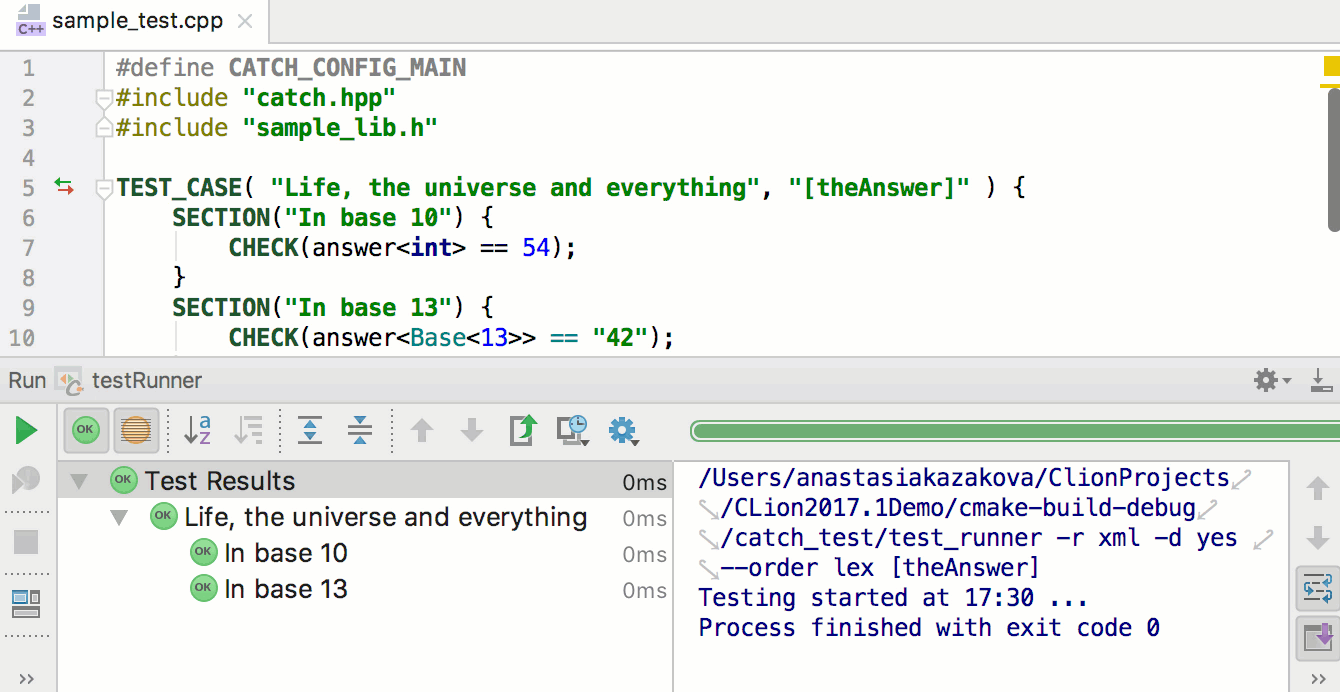
\includegraphics[scale=0.25]{fig/rc6gtest}
\end{figure}
\end{frame}

\subsection{Engineering robustness: Exceptions}
\begin{frame}{Breaking the abstraction}
The central question that goes around with exceptions are:
\begin{center}
	\structure{What if assumptions of an abstraction is broken?}
\end{center}
Note that this should be understand in a broader sense. Any program runs under some assumption. For example, 
\begin{itemize}
	\item There is enough system memory for your program.
	\item There is enough space when you need to create a file.
	\item Input outside \texttt{REQUIRES} clause never happens. 
	\item Your computer have an available Internet connections.
	\item ...
\end{itemize}
All these things constitutes the assumption you made about your abstractions. But it certainly could happen that one (or more) of them are broken. This could due to hardware limitations, or more likely due to an error in programming. 
\end{frame}

\begin{frame}[fragile]{Fail-fast \& ``I give up."}
\alert{There is absolutely no point to save a flawed processess}. This is called the fail-fast fast.
\begin{itemize}
	\item The program is already in an non-recoverable state
	\item It is probably due to a programming error
	\item Error might propagate, crash site far from source.
	\item May corrupt data. Programs can be fixed, data can't.
	\item Best strategy is to quit gracefully.
\end{itemize}
A typical situation:
\begin{minted}{c++}
void foo() {
  int *p = malloc(sizeof(int) * 10);
  // This should always success unless lacking memory
  assert(!p);
  // Do something with p
  free(p);
}
\end{minted}
\end{frame}

\begin{frame}[fragile]{``It's my problem."}
The attempt is to make the function essentially a ``total" function. Essentially this strategy says 
\begin{center}
	\structure{``Invalid inputs are part of my abstraction"}
\end{center}
Which also implies testing for invalid inputs! An (not so good) example:
\begin{minted}{c++}
// Checks if all letters in a string are capital
bool isAllCapital(char* str, int size) {
    int len = strlen(str);
    if (size != len + 1) len = size; // Input validation
    for (int i = 0; i <= len; i++) 
        if (*str < 'A' || *str > 'Z')
            return false;
    return true;
}
\end{minted}
\end{frame}

\begin{frame}{``It's my problem."}
There are some serious problem with this approach:
\begin{itemize}
	\item Function might not have well defined ``default" value. 
	\item It might hard to guess a ``default" value. 
\end{itemize}
Regardless above problem, much more serious problem comes with error propagation. There is probably a reason why this input is valid. It's most likely because you code is incorrect (in some sense) or your running environment is problematic (stack overflowed, for example).

You need to understand whenever you took this approach, you are trying to fix an already ``broken" program, going against the fail-fast principal.

\begin{itemize}
	\item You could end up crashing somewhere far from the root cause.
	\item Your program could behave wired. Since your abstraction includes treatment of ``special cases"
\end{itemize}
\end{frame}

\begin{frame}[fragile]{``It's not my problem"}
The problem of above approaches is significant because they are trying to deal with errors that does not come from themselves. The root cause of these invalid inputs are somewhere else, probably only known by their caller. 

The natural idea would be to find a method to pass the information up the chain of calling, a natural way of doing so is by return \textit{Error Codes}.

There are in general two ways to do so:
\begin{minted}{c}
// Returns negative value if error
int fact1(int n);
// Returns value signifies error, zero indicates no error
// Actual result is put into *rst 
int fact2(int n, int* rst);
\end{minted}
In some cases libraries use a global variable to store the error code of last function call.
\end{frame}

\begin{frame}[fragile]{Problem with error codes}
Both methods have severe draw back:
\begin{minted}{c++}
double tan(double rad);
\end{minted}
Function \texttt{fun} could return anything in \texttt{double}, now what should you use for error code?
\begin{minted}{c++}
int foo(double rad) {
    double rst = 0.0;int err = tan(rad, &rst);
}
\end{minted}
The second makes calling ``unnatural. Also performance drawbacks. 
\begin{itemize}
	\item Error code can be ignored. The worse thing than crashing on errors is an unattended error
	\item Error code needs to be passed up the stream. Sometimes the direct caller also don't have a clue, it needs to pass it on. 
	\item Breaks abstraction.
\end{itemize}
\end{frame}

\begin{frame}[fragile]{Structural Error handling: \texttt{try}, \texttt{catch} and \texttt{throw}}
We know introduce you to \textit{Structural Error Handling}. The following is a try block
\begin{minted}{c++}
// (1)
try {
    // (2) (may throw;)
} catch (const T& e) {
    // (3) ...
}
// (4)
\end{minted}
Just like usually \texttt{if}, \texttt{while} blocks, a \texttt{try} block marks a special control flow, featuring (usually) 2 different code execution paths.
\begin{itemize}
	\item Path 1. Exception raised in (2), we go (1) (2, partial) (3) (4).
	\item Path 2. Normally we go (1) (2) (4).
\end{itemize}
Path 1 assumes the exception is caught. Further discussion on next slide.
\end{frame}

\begin{frame}[fragile]{Structural Error handling: \texttt{try}, \texttt{catch} and \texttt{throw}}
An concrete example. 
\begin{minted}{c++}
try {
    cout << "hello!" << endl; throw 123;
    cout << "Goodbye" << endl;
} catch (int x) {
   cout << "Integer Exception";
}
\end{minted}
Prints \texttt{"Hello//Interger Exception"}
\begin{itemize}
	\item A \texttt{throw} clause raise an exception (of arbitrary type).
	\item When an exception is raise, immediate stop the following execution and go for smallest enclosing \texttt{try} block.
	\item If there isn't one, terminates program.
	\item If there is one, begin matching \texttt{catch} clauses.
	\item If found, we say the error is \textit{handled}, begin executing after \texttt{try}. If not, terminates program.
\end{itemize}
\end{frame}

\begin{frame}[fragile]{Structural Error handling: \texttt{try}, \texttt{catch} and \texttt{throw}}
A try block can be matched no matter how deep in the function. The following example is just for demonstration! \alert{It is NOT a good practice!}
\begin{minted}{c++}
int foo(int n, int prod) {
    if (n == 0) throw prod;
    foo (n - 1, n * prod);
}
int realFact(int n) {
    try {
        foo(n , 1); cout << "LaLaLa";
    } catch (const int& x) {
        cout << "Aloha!" << endl;
        return x;
    }
} // Prints Only "Aloha!".
\end{minted}

\end{frame}

\begin{frame}[fragile]{Structural Error handling: \texttt{try}, \texttt{catch} and \texttt{throw}}
An exception cannnot be overlooked! Unhandeled exception terminates the program.
\begin{minted}{c++}
int fact(int n) { 
    if (n < 0) throw n; 
	if (n == 0) return 1;
	return n * fact(n - 1);
}
int main() { int x = fact(-50); }
\end{minted}
Note we use the word ``Teriminate". There is an difference in \textit{crashing} and \textit{terminating}. 

The first term indicates the program is stopped by force (by the operating system), immediately. 

The second one indicates a seriers events will happen (for example, clearing the buffer of \texttt{cout}). The program terminates (somewhat) gracefully.
\end{frame}

\begin{frame}[fragile]{Structural Error handling: \texttt{try}, \texttt{catch} and \texttt{throw}}
The smallest enclosing \texttt{try} block gets to handle the exception
\begin{minted}{c++}
void foo() {throw -1;}
void bar() {
    try{ foo(); }catch(double e){cout << "bar!";}
    cout << "Slotted Aloha!";
}
void rua() {
    try{ bar(); }catch(int e){cout << "rua!";}
    cout << "Alright!";
}
void baz() {
    try{ rua(); }catch(int e){cout << "baz!";}}
int main() {baz();}
\end{minted}
Above programs prints \texttt{rua!Alright!}. It terminates normally.

\end{frame}

\begin{frame}[fragile]{Structural Error handling: \texttt{try}, \texttt{catch} and \texttt{throw}}
An exception can be rethrown after being caught in a \texttt{catch} block. This is useful since you might need clean up, although you don't known how to deal with the error. It is also possible to throw a different exception.
\begin{minted}{c++}
void foo() {throw -1;}
void bar() {
    int *p = new int(10);
    try{ foo(); }
    catch(...){delete p; cout << "bar!"; throw; }}
void rua() {
    try{ bar(); }catch(int e){cout << "rua!"; throw 1.0;}}
int main() {rua();}
\end{minted}
Above programs prints \texttt{bar!rua!}. It terminates due to an unhandled exception \texttt{1.0}. 
\end{frame}

\begin{frame}[fragile]{Rules for matching for \texttt{catch}}
The rules for matching \texttt{catch} is given as follows:
\begin{enumerate}
	\item First found first match.
	\item Match only with \alert{exact} same type. If the exception is an class instance, also matches with it's base catch.
	\item \texttt{catch(...)} matches everything.
\end{enumerate}
\begin{columns}
	\column{.5\textwidth}

\vspace{-0.2in}
\begin{minted}{c++}
try{int x = 1; throw x;} 
catch(long int li) {
    // No match
} catch (int x) {
    // Match here
} catch (...) {
    // Already matched
}
\end{minted}

	\column{.5\textwidth}
	
\vspace{-0.2in}
\begin{minted}{c++}
try{int x = 1; throw x;}
catch(long int li) {
    // No match
} catch (double x) {
    // No match
} catch (...) {
    // Matched
}
\end{minted}

\end{columns}
\end{frame}

\begin{frame}[fragile]{Exception Hierarchy}
The fact that exception instances can be caught by their base class type is actually very useful in reality. You can catch a ``class" of exceptions while leaving others un touched.
\begin{minted}{c++}
class Exception {};
class IntegerExecption : public Exception {};
class FileExecption    : public Exception {};
class FileNotFound     : public FileExecption {};
class PermissionDenied : public FileExecption {};
void doSomethingToFile(string filename);
void foo(int n) {
    string file = "str" + to_string(n);
    try { doSomethingToFile(file) }
    catch (const FileExecption& e) {
    	cout << "Something wrong with File"; 
} }
\end{minted}
\end{frame}

\begin{frame}{Exception Hierarchy in standard library}
\vspace{-0.2in}
\begin{figure}
	\centering
	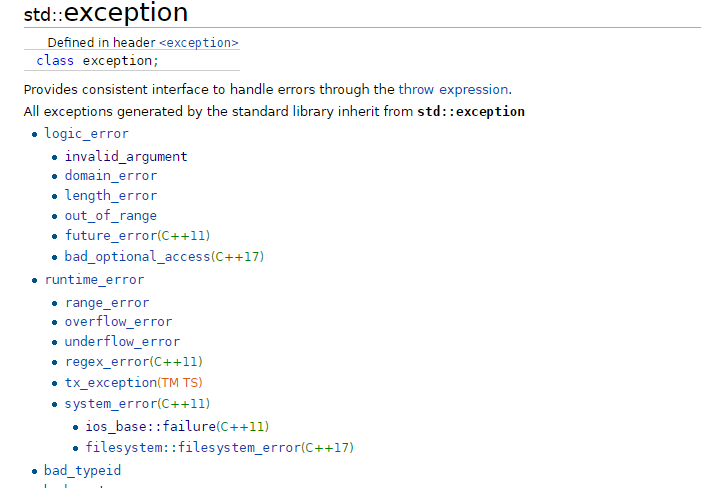
\includegraphics[scale=0.55]{fig/rc6stdexp}
\end{figure}
\end{frame}

\begin{frame}{Tips}
\begin{enumerate}
	\item Throw by value and catch by (const) reference.
	\item \texttt{throw} only on real exceptions
\end{enumerate}
\begin{block}{Throw by value}
	When an exception is raised, the programming is doing sort of recovery. The function that throws the exceptions most likely is going to terminate.
	Thus throwing reference (or address) to local objects won't make sense at the handling site.  
\end{block}
\begin{block}{Catch by (const) reference}
	The very reason that you need to catch exceptions by reference is simply because exceptions can contain virtual functions (polymorphism).
\end{block}
\end{frame}